\chapter{Développement}
\section{Préambule}
À nouveau dans ce TP, nous allons utiliser le mini-logiciel fourni lors du TP 5 pour traiter des images. Sa structure est la même (cf. section 2.1.1 de notre rapport sur les TP 5 et 6). La réprésentation d'une image est également la même (cf. section 2.1.2 de notre rapport sur les TP 5 et 6). Enfin, la conversion en niveaux de gris s'effectue exactement de la même façon (cf. section 2.2.1 de notre rapport sur les TP 5 et 6).

\medskip

\textbf{La différence notable par rapport au TP 5 est qu'ici nous avons la possibilité d'utiliser des \og registres\fg{} MMX de 64bits. Nous avons également accès à de nouvelles instructions très puissantes, qui nous permettent de paralléliser des traitements, tels que la multiplication de plusieurs mots de 16 bits ainsi que leur addition (par exemple).}

\section{Réalisation}
Pour l'écriture du code, nous sommes repartis de ce que nous avions écrit pour le TP 5, en supprimant l'algorithme de conversion et en modifiant quelques lignes pour pouvoir utiliser les instructions MMX.

\medskip

Puis nous avons pu commencer à réfléchir à nos deux algorithmes :
\begin{itemize}
  \item Traitement d'un pixel par itération (chap. \ref{unpixel})
  \item Traitement de deux pixels par itération (chap. \ref{deuxpixels})
\end{itemize}

\chapter{Traitement d'un pixel par itération}
\label{unpixel}
\section{Principe}
MMX propose une instruction très puissante : \lstinline{PMADDWD}. Elle permet de multiplier les mots de 16 bits contenus sur deux registres de 64 bits, puis d'additionner les résultats deux à deux de manière à obtenir deux sommes de 32 bits.
\begin{figure}[!h]
   \centering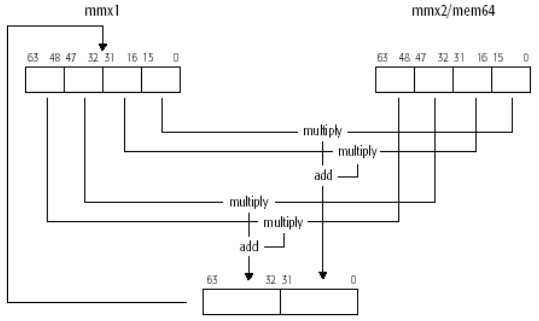
\includegraphics[width=0.7\textwidth]{illustrations/pmaddwd.png}
   \caption{Fonctionnement de PMADDWD}
\end{figure}

Sachant que l'on doit multiplier chaque composante d'un pixel par un c\oe{}fficient (selon la même méthode que dans le TP 5), on peut imaginer stocker sur deux registres MMX différents les c\oe{}fficients et les valeurs des composantes d'un pixel. Il faut donc stocker sur les bits de poids faible de chacun des 4 mots de 16 bits d'un registre les différentes composantes ainsi que les c\oe{}fficients, comme ceci

\begin{center}
64 bits $\underbrace{
    \begin{tabular}{|c|c|c|c||c|c|c|c|}
    \hline
    0x0 & 0x0 & 0x0 & R & 0x0 & G & 0x0 & B \\
    \hline
    \end{tabular}}_{Composantes\ d'un\ pixel}$
\end{center}
\begin{center}
64 bits $\underbrace{
    \begin{tabular}{|c|c|c|c||c|c|c|c|}
    \hline
    0x0 & 0x0 & 0x0 & Coef. R & 0x0 & Coef. G & 0x0 & Coef. B \\
    \hline
    \end{tabular}}_{Coefficients}$
\end{center}

Cependant, pour obtenir une telle \og configuration\fg{} des registres, nous devons utiliser l'instruction \lstinline{PUNPCKLBW} qui permet \og d'éclater\fg{} les octets de deux registres en les espaçant. Nous devrons au préalable placer les c\oe{}fficients dans un registre MMX et les composantes d'un pixel dans un autre registre.

\medskip

Une fois les mutliplications et additions faites grâce à \lstinline{PMADDWD}, nous obtenons quelque chose comme ceci :
\begin{center}
64 bits $\underbrace{
    \begin{tabular}{|c|c|c|c||c|c|c|c|}
    \hline
    0x0 & 0x0 & \multicolumn{2}{c||}{R*Coef} & 0x0 & 0x0 & \multicolumn{2}{c|}{G*Coef+B*Coef} \\
    \hline
    \end{tabular}}_{Composantes\ d'un\ pixel}$
\end{center}

Il ne nous reste plus qu'à additionner les 32 bits de poids fort aux 32 bits de poids faible et à décaler de 8 bits vers la droite pour obtenir notre valeur entière recherchée (pour le gris). Cela se fait aisément grâce aux instructions \lstinline{paddd} et \lstinline{psrlq}. Nous pouvons finalement sauvegarder la nouvelle valeur de notre pixel en mémoire centrale.

\section{Code}

Voici le code final permettant de traiter un pixel par itération :

\assembly
\begin{lstlisting}
; ...
; CODE fourni

    dec ecx
    imul ecx, 4

    ; Copie des constantes multipliées par 256 dans mm1
    mov eax, 150d ; GREEN
    mov ah, 77d ; RED
    shl eax, 8
    mov al, 29d ; BLUE
    movd mm1, eax

    pxor mm3, mm3 ; RESET
    punpcklbw mm1, mm3 ; "Eclatement" des coefficients


boucle:
    movd mm0, dword ptr [esi+ecx] ; Copie du pixel source (32 bits)
    
    pxor mm2, mm2 ; RESET
    punpcklbw mm0, mm2 ; "Eclatement" des composantes R, G et B
    pmaddwd mm0, mm1 ; Multiplication par les coefficients et addition
    movq mm2, mm0 ; Copie de mm0 dans mm2
    psrlq mm2, 32 ; On ne conserve que les 32 bits de poids fort (donc R*Coef)
    paddd mm0, mm2 ; Addition de R*Coef sur mm2 avec (G*Coef + B*Coef) sur mm0
    psrld mm0, 8 ; Décalage d'un octet vers la droite
    movd eax, mm0 ; On sauvegarde les 32 bits de poids faible de mm0 dans eax (donc la valeur du gris)

    mov [edi+ecx], eax ; On sauvegarde la valeur du pixel que l'on copie dans l'image de destination

    sub ecx, 4 ; Pixel suivant
    jne boucle ; On continue tant qu'on n'a pas traité tous les pixels


; CODE fourni
; ...
\end{lstlisting}

\bigskip

\textbf{Attention :} Ce code ne fonctionne pas pour une image contenant un seul pixel. Pour corriger cela, il faudrait modifier le saut conditionnel de la fin. Néanmoins, à la fin de ce rapport, un code est proposé : il fonctionne pour une image ayant 2n+1 pixels (avec n $\geq$ 0) et traite deux pixels à la fois.


\section{Comparaison des performances par rapport au TP 5}

\begin{figure}[!h]
   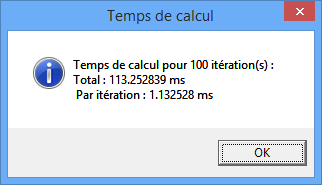
\includegraphics[width=0.5\textwidth]{screens/assembly.png}
   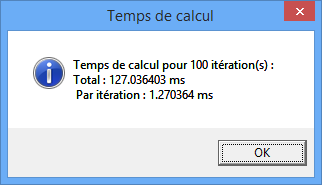
\includegraphics[width=0.5\textwidth]{screens/mmx_1px.png}
   \caption{À gauche x86, à droite x86 avec MMX}
\end{figure}

On constate des performances légèrement inférieures à ce que l'on avait obtenu lors du TP 5. Cela peut s'expliquer par un nombre d'instructions un peu plus élevé dans notre algorithme du TP 6 par rapport à celui du TP 5. La puissance des instructions MMX n'est pas exploitée convenablement. Il convient donc de traiter maintenant deux pixels par itération de manière à augmenter significativement les performances.

\chapter{Traitement de deux pixels par itération}
\label{deuxpixels}
\section{En traitant une image avec un nombre pair de pixels}
\subsection{Principe}
Le principe est le même que pour un pixel, sauf que l'on va traiter en même temps deux pixels.

\medskip

Pour cela, à chaque itération, il suffit de copier deux pixels sur un registre MMX (un pixel dans les 32 bits de poids fort, un autre dans les 32 bits de poids faible). Les composantes R, G et B de chaque pixel sont ensuites \og éclatées\fg{} (espacées) sur deux registres différents à l'aide d'instructions de type \textbf{unpack}.

\medskip

Ensuite, les composantes de chaque pixel sont multipliées par les bons c\oe{}fficients à l'aide de l'instruction \lstinline{pmaddwd}. Puis, R*Coef est additionné à (G*Coef + B*Coef) pour chaque pixel, comme dans l'algorithme qui traite un pixel un par un. \textbf{Ce traitement est le même que celui du chapitre \ref{unpixel}}.

\medskip

Finalement, les deux sommes sont remises dans un registre MMX (une somme dans les 32 bits de poids fort, l'autre dans les 32 bits de poids faible, en faisant attention à ne pas inverser les deux pixels). Et le registre est copié en mémoire centrale, dans l'image de destination. Le code détaillé ci-dessous explique tout cela grâce à des commentaires.

\subsection{Code}

\begin{lstlisting}
; ...
; CODE fourni

    dec ecx
    imul ecx,4

    ; Copie des constantes dans mm1
    mov eax, 150d ; GREEN
    mov ah, 77d ; RED
    shl eax, 8
    mov al, 29d ; BLUE
    movd mm1, eax

    pxor mm3, mm3
    punpcklbw mm1, mm3

    sub ecx, 4 ; On veut traiter le pixel 0 ET le pixel 1, donc on avance pour ne pas lire le pixel 0 et le "pixel -1" (qui n'existe pas)

bouclee:
    movq mm0, qword ptr [esi+ecx] ; On charge deux pixels d'un coup (64 bits)

    pxor mm2, mm2 ; RESET
    punpckhbw mm2, mm0 ; Espacement des composantes R, G et B du pixel contenu dans les bits de poids fort (high)
    psrlw mm2, 8 ; On met les composantes dans les bits de poids faible des mots de 16 bits

    punpcklbw mm0, mm3 ; Espacement des composantes R, G et B du pixel contenu dans les bits de poids faible (low)

    pmaddwd mm0, mm1 ; Multiplication par les coefficients et addition
    pmaddwd mm2, mm1 ; Multiplication par les coefficients et addition

    movq mm4, mm0 ; Copie de mm0 dans mm4

    punpckldq mm4, mm2 ; On met les composantes G*Coef + B*Coef de chaque pixel cote a cote dans mm4
    punpckhdq mm0, mm2 ; On met la composante R*Coef de chaque pixel côte à côte dans mm0

    paddd mm4, mm0 ; Pour chaque pixel, addition de R*Coef avec (G*Coef + B*Coef)
    psrld mm4, 8 ; On ne garde que la partie entière de la valeur du gris obtenue (décalage de 8 bits)

    movq qword ptr [edi+ecx], mm4 ; On sauvegarde la valeur du pixel que l'on copie dans l'image de destination

    sub ecx,8 ; On saute 2 pixels à chaque fois
    jne bouclee ; On continue tant qu'on n'a pas tout traité

; CODE fourni
; ...
\end{lstlisting}

\subsection{Comparaison des performances par rapport au traitement d'un pixel par itération}

\begin{figure}[!h]
   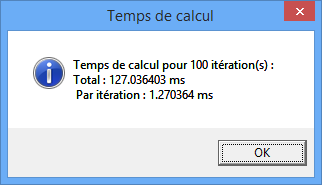
\includegraphics[width=0.5\textwidth]{screens/mmx_1px.png}
   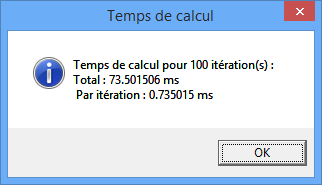
\includegraphics[width=0.5\textwidth]{screens/mmx_2px.png}
   \caption{À gauche un pixel par itération, à droite deux pixels par itération}
\end{figure}

On constante un gain très important de performance : il faut presque deux fois moins de temps pour traiter une image. Cela s'explique par le fait que l'on exploite pleinement la puissance des instructions MMX ici, en parallélisant les traitements.

\section{En traitant une image avec n'importe quel nombre de pixels}

Le code précédent souffre d'un problème : si l'image contient un nombre de pixels impair, à un moment le programme accèdera à de la mémoire qu'il n'est pas sensé utiliser.

\medskip

\noindent Il faut donc prendre en considération deux cas :
\begin{itemize}
  \item L'image possède un seul pixel
  \item L'image possède 2n+1 pixels (avec n > 0)
\end{itemize}

\medskip

Cela se fait aisément en ajoutant des sauts conditionnels au début du programme et à la fin des boucles, comme ceci :

\begin{lstlisting}
; ...

    dec ecx
    imul ecx,4

    ; Copie des constantes dans mm1
    ; ...

    pxor mm3, mm3
    punpcklbw mm1, mm3

    ; Si l'image fait AU MOINS 2 pixels, ecx sera supérieur à 0 car ecx = (nombre de pixels - 1) * 4
    cmp ecx, 0
    ja twopixels
    ; Sinon il n'y a qu'un seul pixel

unpixel:
    movd mm0, dword ptr [esi+ecx] ; 32 bits

    ; ...

    mov [edi+ecx], eax ; On sauvegarde la valeur du pixel que l'on copie dans l'image de destination

    jmp fin ; C'était le dernier pixel à traiter

twopixels:
    sub ecx, 4

bouclee:
    movq mm0, qword ptr [esi+ecx] ; On charge deux pixels d'un coup (64 bits)

    ; ...

    movq qword ptr [edi+ecx], mm4 ; On sauvegarde la valeur du pixel que l'on copie dans l'image de destination

    sub ecx, 4
    cmp ecx, 0
    je unpixel ; S'il reste QU'UN SEUL pixel à traiter, on appelle l'algo à l'étiquette 'unpixel'
    jl fin ; Si c'est inférieur à 0, on a tout traité
    sub ecx, 4 ; Sinon il reste au minimum 2 pixels à traiter
    jmp bouclee ; Et donc on traite les 2 pixels suivants

fin:

; ...
\end{lstlisting}

\noindent Le code complet de cette partie est trouvable en annexes.